\chapter{Theory}
\label{chap:theo}




\section{Quadcopter Modelling}

\par{test}

\todo{fundamental physics}



\todo{particle simulation}



\section{Vrep}
\label{sec:theoryVrep}
V-REP is a versatile, highly customisable simulation environment, mainly developed for robots. It provides a rich set of functionolaties which we use only a part off.  We make use of it's integration of the bullet physics engine, including a particle simulation, it's external Java API, the communication structure via signals, the possibility of Lua scripting inside the simulation, it's provided sensor-simulation and the scene visualisation.
\begin{figure}[h!]
 \begin{center}
  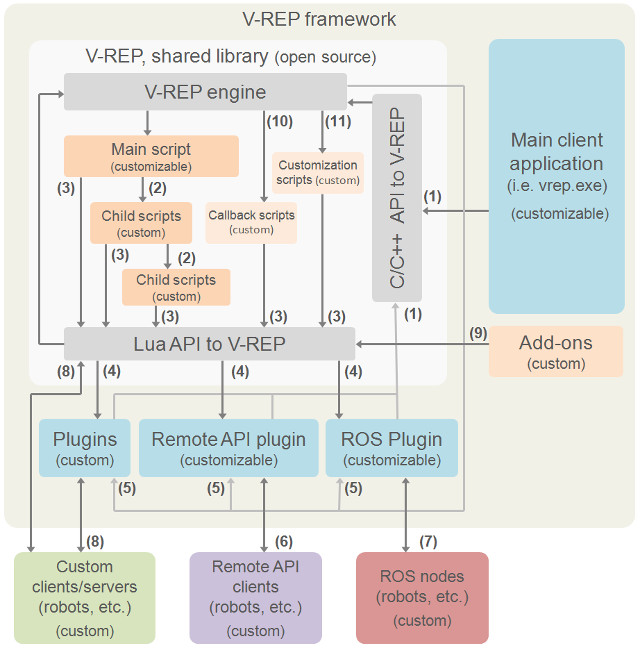
\includegraphics[scale=0.45]{vrepStruct.jpg}
 \end{center}
  \caption{Structure of the VREP-framework \url{http://www.coppeliarobotics.com/helpFiles/en/images/writingCode1.jpg} 13.10.2015 \label{fig:vrepStruct}}
\end{figure}

The V-REP main client application provides the basis vor the simulation. V-REP bases on scenes in which the simulation settings and scenes are saved. To run a simulation, the necessary objects need to be added to the scene. An object can be a dummy object with no physical properties, a 3-D shape either imported via an .stl-file or created directly in V-REP. V-REP already provides a library of objects, starting with sensors and continuing with whole robots. An example are force sensors which can be used to connect object. Then, the force sensor transmits the resulting forces and torques during the simulation and can be set to break when exceeding a certain threshold. Connecting objects without force sensors can be used to separate physical simulation and visual representation. The connection becomes static, so a complex, but visually appealing mesh shape can be attached to a simpler shape with appropriate physical parameters. Thereby, physical simulation calculation are performantly done on the simple, and as V-REP provides several visibility layers, the user sees only the complex shape.

V-REP provides several possibilities to extend the simulation programmatically. The easiest and best integrated way are Lua-scripts. Lua scripts can be attached to simulation objects and are handles within the simulation environment. When choosing non-threaded child scripts, they get executed every simulation step and can influence scene objects via a comprehensive API. A V-REP simulation step consists of several sections. To execute parts of the script only at certain points, the current simulation status can be checked before executing code.  The downside of these Lua-scripts is, that they are stored inside the binary scene file. Thus, it's difficult to put them under version control or do collaborative work. As the Lua-Engine inside V-REP provides full Lua support, this can be avoided by using the internal scripts only to import and call the actual scripts that are stored outside the scene. In section \ref{sec:implSoftware} is described how we handled this problem in detail.

If Lua doesn't offer the needed performance or functionalities, the second way to build deeply integrated software is the internal C++ API for plugins.  The most flexible, but least performant way is the remote API of V-REP. Providing an API for Java, Matlab, Python and Urbi, it interacts with many programming languages. However, the functionality provided by the remote API is limited compared to the internal API for Lua or C++. For the remote API, V-REP needs to start a server that the client connects to. This is also possible over network, so the computation load can be distributed between different machines.

For communication inside V-REP, global custom variables can be used. As the access to those is not supported by the remote API, a more flexible way are \emph{Signals}. \emph{Signals} can be of String, Integer or Float type and are globally accessible  in the current scene. 










\section{Communication V-REP-Quadrocopters}
\label{sec:comm}
\textbf{\textit{Goal}:} our mixed reality simulation needs a dependable link of communication between the V-REP simulation environment and the flying quadrocopters. The Quadcopter needs to stream its telemetry data in real-time to the V-REP, and the reverse communication is needed as well.\\
The simulated quadrocopters that we have in the V-REP are divided into two categories: real and virtual representations.\\ 
The real are replicating the physical flying quadrocopters. They should perform the same flying manoeuvres as those flying in the real environment. In order to make the model replicate this behaviour, the flying quadrocopter must send its linear and angular velocity, its pitch yaw and row and other parameters in real time to its representation model in V-REP. The simulation model should also send the readings from its proximity sensors to the flying quadcopter thus providing it with information from a virtual sensor. \\
The virtual quadrocopters are purely simulation quadcopter objects, that exist only in the V-REP simulation environment. Their purpose is to interact with the real quadrocopters for example to avoid collisions and thus making the first steps in the swarm research. The virtual quadrocopters have to be seen in the Paparazzi ground station as if they are real physical quadrocopters. It means that all the ground station agents like message logger, the signal plotting, attitude indicator, artificial horizon and other displays have to be updated with adequate information coming from the virtual quadrocopters in the V-REP.

The communication between the V-REP quadrocopter models and the physical quadrocopters passes through several software components, which are depicted on figure \ref{fig:communication} and discussed in the next chapters.

\begin{figure}[h!]
 \begin{center}
  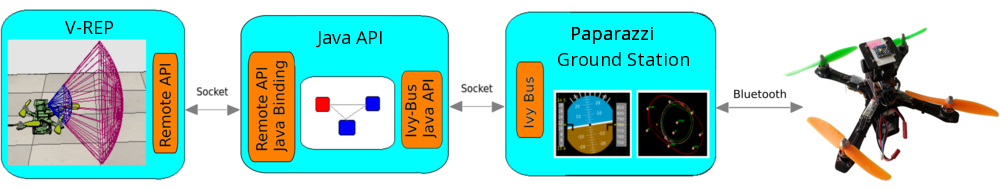
\includegraphics[scale=0.15]{communication.png}
 \end{center}
  \caption{communication V-REP - Quadrocopter\label{fig:communication}}
\end{figure}

\subsection{V-REP Remote API}
V-REP provides several means of communication with an external application. One of them is the Remote API, which allows to control a simulation (or the simulator itself) from an external application or a remote hardware (e.g. real robot, remote computer, etc.). The V-REP remote API is composed by approximately one hundred functions that can be called from a C/C++ application, a Python script, a Java application, a Matlab/Octave program, an Urbi script, or a Lua script. The remote API functions are interacting with V-REP via socket communication in a way that reduces lag and network load to a great extent.

\subsection{Java API}
Java API is the external program, that we have implemented to communicate with V-REP through the Remote API.
We have chosen to implement our external program, communicating with the V-REP, in the Java programming language regarding the following advantages: Java's platform independence allows to run the external program even on different machine with different operating system than the one used for running the V-REP environment.  Java is object-orientated which favours the use of design patterns and highly abstraction layers, which allows us to write an API that is modular, reusable and can later be easily extended to support other mixed-reality scenarious. The implementation and architecture of the Java API is duscussed in details in \ref{sec:implementation}. The purpose of the Java application is to serve as a communicating bridge between the Paparazzi Ground Station and the V-REP. It detects all quadrocopters in the V-REP simulation, builds their virtual representations and feeds the models with real-time data.

\subsection{Ivy Bus}
Ivy Bus is a simple protocol and a set of open-source (LGPL) libraries and programs that allows applications to broadcast information through text messages, with a subscription mechanism based on regular expressions. Ivy libraries are available in C, C++, Java, Python and Perl, on Windows and Unix boxes and on Macs. \\
The Paparazzi Ground Station uses the Ivy Bus as a means of communication between the different software components. Figure \ref{fig:paparazziGS} depicts the communication structure in the Paparazzi Ground Station, in which the different agents communicate with each other by sending messages on the Ivy-Bus.

\begin{figure}[h!]
 \begin{center}
  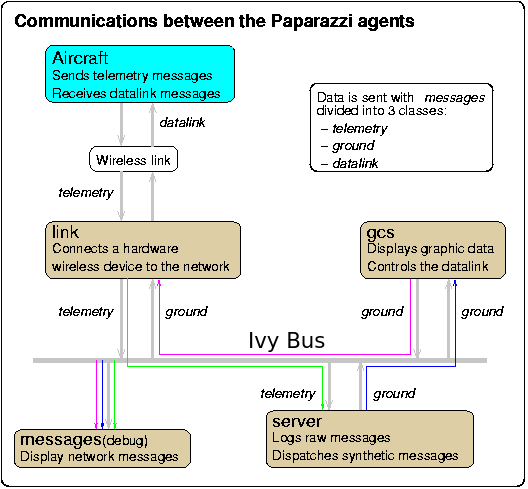
\includegraphics[scale=0.7]{paparazzi_gs.png}
 \end{center}
  \caption{Ivy-Bus in Paparazzi Ground Station\label{fig:paparazziGS}}
\end{figure}

The UAV (in blue) is streaming its telemetry data to the ground control station, which is received by the link. The \textbf{link} agent manages the ground-based radio modem and distributes the received messages to the other agents across the Ivy-Bus.

The Ivy Bus is an example of a publisher-subscriber protocol, in which senders of messages, called publishers, does not  explicitly specify the address of the receiver, but just send the message on one, shared by all nodes, bus. The recipients, called subscribers, which are interested in the message will accept it and the others will ignore it. The publisher-subscriber is a many to many communication model in which publishers are loosely coupled to subscribers - there is no space, flow and time coupling. This means that the publishers does not have to know the addresses of the subscribers and even does not need to know of their existence. Each can operate normally without the other and can continue its thread of execution regardless if the subscriber has received the message or not. It also provides scalability, which means that we can “attach” our Java API to the Ivy-Bus and start publishing and listening for messages without changing any line of source code in the Paparazzi Ground Station software.

In the publisher-subscriber model, subscribers typically receive only a subset of the total messages published. The process of selecting messages for reception and processing is called filtering. There are two common forms of filtering: topic-based and content-based.
In a topic-based system, messages are published to "topics" or named logical channels. Subscribers in a topic-based system will receive all messages published to the topics to which they subscribe, and all subscribers to a topic will receive the same messages. The publisher is responsible for defining the classes of messages to which subscribers can subscribe.
In a content-based system, messages are only delivered to a subscriber if the attributes or content of those messages match constraints defined by the subscriber. The subscriber is responsible for classifying the messages. Both filtering techniques are depicted in figures \ref{fig:pubsubsc_topic_based} and \ref{fig:pubsubsc_content_based}.

The Ivy Bus is a content-based publisher-subscriber and uses regular expressions for the message filtering.

\begin{figure}[!tbp]
  \centering
  \begin{minipage}[b]{0.4\textwidth}
    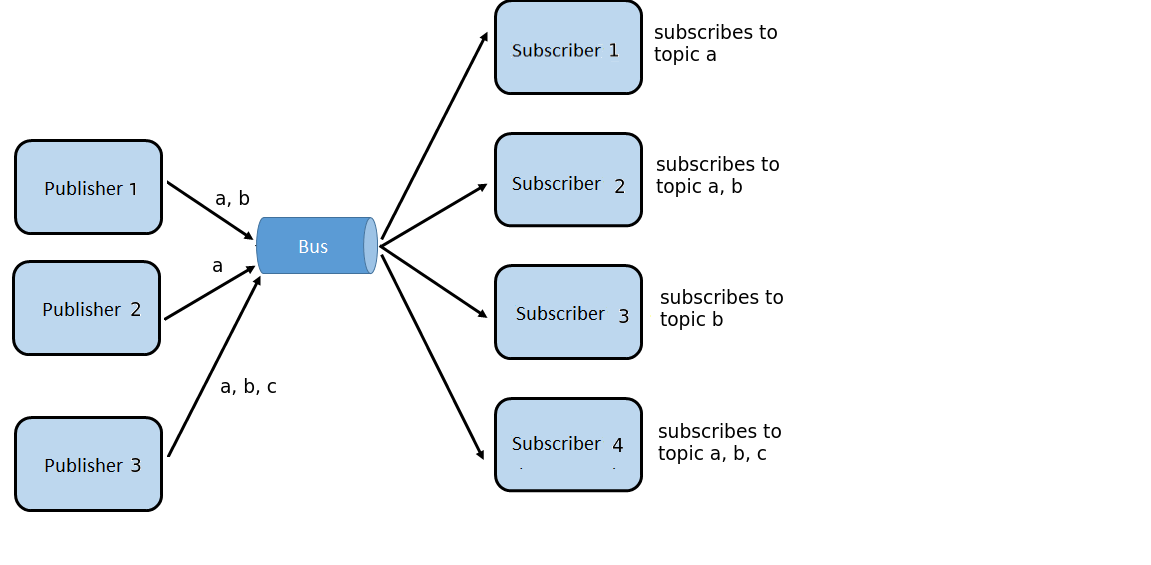
\includegraphics[scale=0.4]{pubsubsc_topic_based.png}
    \caption{Topic-based publisher-subscriber \label{fig:pubsubsc_content_based}}
  \end{minipage}
  \hfill
  \begin{minipage}[b]{0.4\textwidth}
    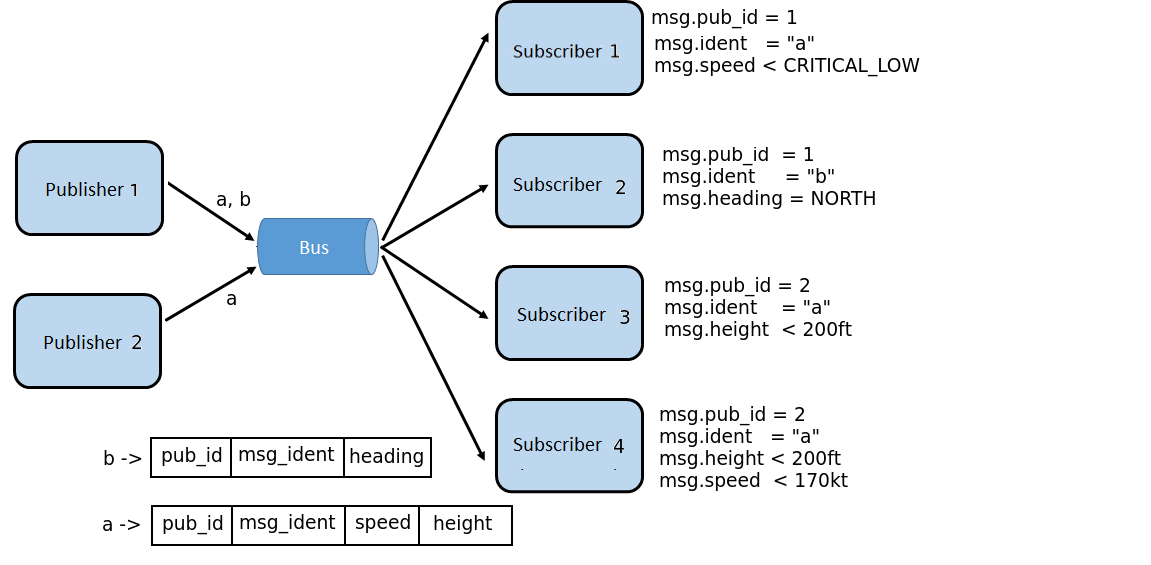
\includegraphics[scale=0.4]{pubsubsc_content_based.png}
    \caption{Content-based publisher-subscriber \label{fig:pubsubsc_topic_based}}
  \end{minipage}
\end{figure}

\subsection{Communication}
\label{sec:communication}

The communication between V-REP and the quadrocopters passes through the Java API, which serves as a bridge between them. In fact the Java API does not communicate directly with the quadrocopter, but connects to the Ivy-Bus in the Paparazzi GS and can thus subscribe to the messages caring the telemetry data and also publish messages which will eventually be send to the quadrocopter by the link agent. On the other hand it uses the V-REP Remote-API to exchange information and provide the V-REP quadrocopter models with the data retrieved from the Ivy-Bus messages.\\ 
Since we wanted to create a modular and reusable API, that can be used for other mixed-reality scenarios, the Java API was created with the idea in mind to be distributed, modular and rely on many abstraction layers.\\ 
The API development has followed the requirement-driven principles and its main tasks are described in the following paragraphs. The implementation of the described bellow requirements in described in \ref{sec:commImplementation} of \ref{sec:implementation}.

\subsubsection{V-REP-Remote API specific requirements}
\label{sec:requirementsVREP}

Below is a description of the requirements for the Java API which is responsible for the connection and communication with the V-REP environment. Its implementation is described in \ref{sec:vrepImplementation} of \ref{sec:implementation}.

\paragraph{Connection to V-REP through the Remote API}

There should be implemented a mechanism that enables to establish connection to the V-REP simulation. The connection should be able to be disconnected and reconnected at any time. Since the Remote API is based on a socket connection, it should be possible to connect to a V-REP server, situated on another machine, by specifying its IP address and port number. This will allow to run the V-REP simulation on a remote, powerful computer and thus release the local computer from having to deal with the simulation and communication program at the same time.

\paragraph{V-REP scene object and scene representation}\label{sceneobject}
The main elements in V-REP that are used for building a simulation scene are scene objects (objects in short). Objects are visible in the scene hierarchy and in the scene view. In the scene view, objects have a three dimensional representation. Some of the object types are: shape, joint, proximity sensors, vision sensors and others. The shape object is a rigid mesh that is composed of triangular faces. Our quadrocopters are represented as a shape objects in the V-REP scene. But is also contains four infrared sensors which are of type proximity sensor object. So the quadrocopter is represented as a complex scene object. 
The V-REP scene objects have to be represented as individual classes in order to be able to easily distinguish them and work with their properties. The class representing the scene object must have as fields the properties describing the simulation object - liniar and angular velocity, position and orientation. The V-REP scene object hierarchy should also be implemented by using inheritance and composition object oriented techniques. \\
The Java API should provide methods to retrieve all scene objects from the V-REP scene and store them in a virtual scene representation for later use.\\
Since our quadrocopters are represented as shape objects and typically a V-REP scene contains at least 20 shape objects by default, there should be implemented a scanner that retrieves the quadrocopters from the scene. The scanner must be able to retrieve the virtual and real quadrocopters in a separate containers.

\paragraph{Continuous data exchange between quadrocopter instances and V-REP}

As mentioned at the beginning of \ref{sec:comm} we divide our quadrocopters in virtual and real representation. The virtual representations exist only in the V-REP scene, but they have to be visible in the paparazzi ground station as if they are real flying drones. It means that all the quadrocopter flying parameters have to be sent to the paparazzi ground station as messages. It becomes clear that the virtual quadrocopters have to be provided continuously with live data from the V-REP - linear/angular velocity, position and orientation. The real quadrocopter representations does not need to be provided with V-REP parameters, since its velocity, orientation and height are coming from the physical flying drone, but it has to be provided with data from its proximity sensor scene objects. The update with V-REP data should have a frequency equal to the simulation step used - 50 ms by default.\\
The real quadrocopter representation get provided with velocity, orientation and height from the physical flying quadrocopter and this data have to be provided to the V-REP quadrocopter object in order to fly like the physical one. This is the inverse communication from quadrocopter to V-REP and is realized with V-REP signaling mechanism. The update is done each time a new message has been received by the physical drone and its frequency depends on how often the messages are streamed from the copter and the communication latency. In order to achieve a realistic flying manuevers and have minimum drift the update should not exceed 20 ms.

\subsubsection{Ivy Bus specific requirements}
\label{sec:requirementsIVYBus}
\paragraph{Ivy Bus connection}
Each participant which wants to exchange information on the Ivy-Bus is described as a singular and independent bus node. In our program the participants that want to exchange data on the Ivy-Bus are the virtual and real representations of the quadrocopters. There should be designed a class, which allows the connecting on the bus, publishing and subscribing to messages. The quadrocopter representations have to inherit from it or composite it and thus become independent bus nodes.

\paragraph{Message retrieval and subscription}

All the messages that the paparazzi software uses are described in a xml file called \textit{messages.xml}, residing in the \textit{/paparazzi/conf/} directory. The following listing is an example of the messages file containing two messages.

\begin{lstlisting}[basicstyle=\tiny]
<msg_class name="telemetry">
 <message name="AIRSPEED" id="54">
    <field name="airspeed" type="float" unit="m/s"/>
    <field name="airspeed_sp" type="float" unit="m/s"/>
    <field name="airspeed_cnt" type="float" unit="m/s"/>
    <field name="groundspeed_sp" type="float" unit="m/s"/>
  </message>
  
  <message name="SONAR_ARRAY" id="216">
	<field name="sonar_front" type="uint16" alt_unit="cm"/>
	<field name="sonar_right" type="uint16" alt_unit="cm"/>
	<field name="sonar_back" type="uint16" alt_unit="cm"/>
	<field name="sonar_left" type="uint16" alt_unit="cm"/>
  </message>
	
	  . . . . 
	  
</msg_class>
\end{lstlisting}

In order to make the subscription and publishing of messages on the bus easier, each message should be represented as a corresponding class containing the message fields with its type and units.

There should be implemented a class, which reads the \textit{messages.xml} file and creates an instance of the message class for each message. \\
Once the messages are retrieved, the Ivy-Bus node should be capable of subscribing and publishing of any of the retrieved messages. The subscription should by dynamic and allow to subscribe to a new messages even at runtime. \\
Once a message has been received, the Ivy-Bus node should provide the instance of the received message and its fields should contain the actual sensor values.\\
Since our mixed reality scenario can involve many flying quadrocopters, there will be published the same messages but from different copters. In this case the messages are identified with the drone id number.
Another requirement is that the Ivy-Bus node have to subscribe just to the messages published from the copter that it was assigned to and not receive the same messages from the other copters.



% example for definition    
% \begin{definitionnonum}[Softwarearchitektur ]
% Die Softwarearchitektur repräsentiert alle Softwarekomponenten und deren Interaktionen in einer hierarchischen Struktur. Es werden sowohl statische Aspekte wie Schnittstellen und Datenpfade zwischen Softwarekomponenten, als auch dynamische Aspekte wie Prozessabläufe und zeitliches Verhalten beschrieben.
% \end{definitionnonum} 
 

  
%  example for bulletpoints
%\begin{itemize}    
%	\item{(überarbeiteter) Sicherheitsplan nach ISO 26262-6:2011, 5.5.1}
%	\item{Design- und Programmierrichtlinien für Programmier- und Modellierungssprachen nach ISO 26262-6:2011, 5.5.5}
%	\item{Hardware-Software-Interfacespezifikation nach ISO 26262-4:2011, 7.5.6}
%	\item{Software-Sicherheitsanforderungen nach ISO 26262-6:2011, 6.5.1}
%	\item{(überarbeiteter) Software-Verifizierungsplan nach  ISO 26262-6:2011, 6.5.3}
%	\item{Software-Verifizierungsbericht nach ISO 26262-6:2011, 6.5.4}
%\end{itemize}

 
%example for table    
% \begin{table}[h]
%      \centering
%    \caption{7.4.1 Notationen für Softwarearchitekturen\cite{iso6}}
%    \begin{tabular}{|c|l|c|c|c|c|}
%      \hline
%     \multicolumn{2}{|c|}{\multirow{2}{*}{Methoden}} & \multicolumn{4}{|c|}{ASIL}\\
%      \multicolumn{2}{|c|}{} &A & B & C & D\\
%      \hline
%       1a & Informelle Notationen & ++ & ++ & + & +\\
%      \hline
%       1b & Semi-formale Notationen & + & ++ & ++ & ++\\
%      \hline
%        1c & Formale Notationen & + & + & + & +\\
% 
%      \hline
%      \end{tabular}
%      \label{tab:archDescr}
%\end{table}
